\documentclass[12pt,a4paper]{article}
\usepackage[utf8]{inputenc}
\usepackage[T2A]{fontenc}
\usepackage[ukrainian]{babel}
\usepackage{geometry}
\usepackage{amsmath}
\usepackage{amssymb}
\usepackage{graphicx}
\usepackage{float}
\usepackage{array}
\usepackage{booktabs}
\usepackage{xcolor}
\usepackage{listings}
\usepackage{fancyhdr}
\usepackage{hyperref}

\geometry{left=2cm, right=2cm, top=2cm, bottom=2cm}
\pagestyle{fancy}
\fancyhf{}
\fancyhead[L]{Розпізнавання образів}
\fancyhead[R]{Лабораторна робота 1}
\fancyfoot[C]{\thepage}
\setlength{\headheight}{15pt}

\setlength{\parindent}{0.5cm}
\linespread{1.5}

%================ ТИТУЛЬНА СТОРІНКА ================
\begin{document}

\begin{titlepage}
\centering
{\Large \textbf{КИЇВСЬКИЙ НАЦІОНАЛЬНИЙ УНІВЕРСИСТЕТ\\
ІМЕНІ ТАРАСА ШЕВЧЕНКА}}

\vspace{2cm}

{\large Факультет комп'ютерних наук та кібернетики}

\vspace{3cm}

{\Large \textbf{ЛАБОРАТОРНА РОБОТА 1}}

\vspace{0.5cm}

{\large \textbf{Розпізнавання образів}}

\vspace{2cm}

{\large \textbf{Побудова системи вкладених еліпсів\\
та оцінка ймовірності належності точок}}

\vspace{3cm}

{\large \textbf{Виконав:} студент групи ПМ}

\vspace{0.5cm}

{\Large \textbf{Кіщук Ярослав Ярославович}}

\vspace{3cm}

{\large \textbf{Київ} -- 2026}

\end{titlepage}

\newpage
\tableofcontents
\newpage

%================ ВСТУП ================
\section{Мета та завдання роботи}

\subsection{Мета}
Розробити алгоритм побудови системи вкладених еліпсів на основі множини вихідних точок та здійснити оцінку ймовірності належності тестових точок до цієї системи.

\subsection{Завдання}

Реалізувати наступні етапи алгоритму:

\begin{enumerate}
    \item Генерувати точки двох типів: основні точки для побудови еліпсів та тестові точки
    \item Знайти дві найвіддаленіші точки першого типу на опуклій оболонці
    \item Знайти дві найвіддаленіші точки по різні боки від прямої, що їх з'єднує
    \item Привести область до квадратної форми через масштабування
    \item Побудувати систему вкладених кіл в центрі квадратної області
    \item Визначити, у скількох колах знаходиться кожна тестова точка
    \item Здійснити зворотне масштабування та поворот для отримання системи еліпсів
    \item Розрахувати площи еліпсів та ймовірності належності тестових точок
\end{enumerate}

%================ ТЕОРЕТИЧНІ ОСНОВИ ================
\section{Теоретичні основи}

\subsection{Опукла оболонка}

Опукла оболонка множини точок — це найменша опукла множина, що містить всі точки. Для знаходження використовується алгоритм Грехема (Graham Scan), який працює за часом $O(n \log n)$ [1, 2].

\subsection{Система координат}

На першому етапі координатна система повертається таким чином, щоб пряма, що з'єднує дві найвіддаленіші точки, співпадала з горизонтальною віссю. Матриця повороту на кут $-\theta$:

\begin{equation}
R = \begin{pmatrix} \cos\theta & \sin\theta \\ -\sin\theta & \cos\theta \end{pmatrix}
\end{equation}

де $\theta = \arctan2(dy, dx)$ — кут напрямку прямої до осі $Ox$ [3].

\subsection{Приведення до квадратної області}

Область масштабується так, щоб ширина дорівнювала висоті, а центр залишався на місці:

\begin{equation}
x'_i = \frac{x_i - x_c}{k} + x_c, \quad k = \frac{\max(\text{ширина}, \text{висота})}{\min(\text{ширина}, \text{висота})}
\end{equation}

Такий афінний перетворювач зберігає порядок вкладеності контурів та використовується для нормалізації форми області [3, 4].

\subsection{Система вкладених кіл та еліпсів}

У центрі квадратної області будується система концентричних кіл з радіусами, що дорівнюють відстаням від центру до кожної точки множини:

\begin{equation}
r_1 \leq r_2 \leq \ldots \leq r_n
\end{equation}

При зворотному масштабуванні кола перетворюються на еліпси з піввісями:
\begin{align}
a &= k \cdot r \quad \text{(якщо стискали по } x\text{)} \\
b &= r
\end{align}

Площа еліпса:
\begin{equation}
S = \pi \cdot a \cdot b
\end{equation}

Формула площі еліпса та геометричний зв'язок між колом і еліпсом після неоднорідного масштабування є класичним результатом аналітичної геометрії [5].

\subsection{Ймовірність належності}

Для кожної тестової точки визначається номер $m$ максимального кола, що її містить. Ймовірність належності розраховується за формулою:

\begin{equation}
P = \frac{m - 1}{n + 1}
\end{equation}

де $n$ — загальна кількість еліпсів. Рангове оцінювання належності через порядковий номер вкладеного контуру відповідає ідеї непараметричної оцінки за емпіричним порядком [4].

\textbf{Граничні випадки:}
\begin{itemize}
    \item $m = 0$ (точка в центрі): $P = 0$
    \item $m \geq n$ (точка зовні всіх кіл): $P = 1$
    \item $0 < m < n$ (нормальний випадок): $P = \frac{m-1}{n+1}$
\end{itemize}

%================ АЛГОРИТМ ================
\section{Описання алгоритму та реалізація}

\subsection{Параметри роботи}

\begin{table}[H]
\centering
\begin{tabular}{|l|r|}
\toprule
\textbf{Параметр} & \textbf{Значення} \\
\midrule
Кількість основних точок ($n_{main}$) & 150 \\
Кількість тестових точок ($n_{test}$) & 30 \\
Діапазон $x$ & $[-50, 50]$ \\
Діапазон $y$ & $[-22, 22]$ \\
Seed (для відтворюваності) & 42 \\
\bottomrule
\end{tabular}
\caption{Параметри генерації точок}
\end{table}

\subsection{Крок 1: Генерація вихідних точок}

Генеруються два набори точок з рівномірним розподілом:
\begin{itemize}
    \item 150 основних точок для побудови системи еліпсів
    \item 30 тестових точок для класифікації
\end{itemize}

\begin{figure}[H]
\centering
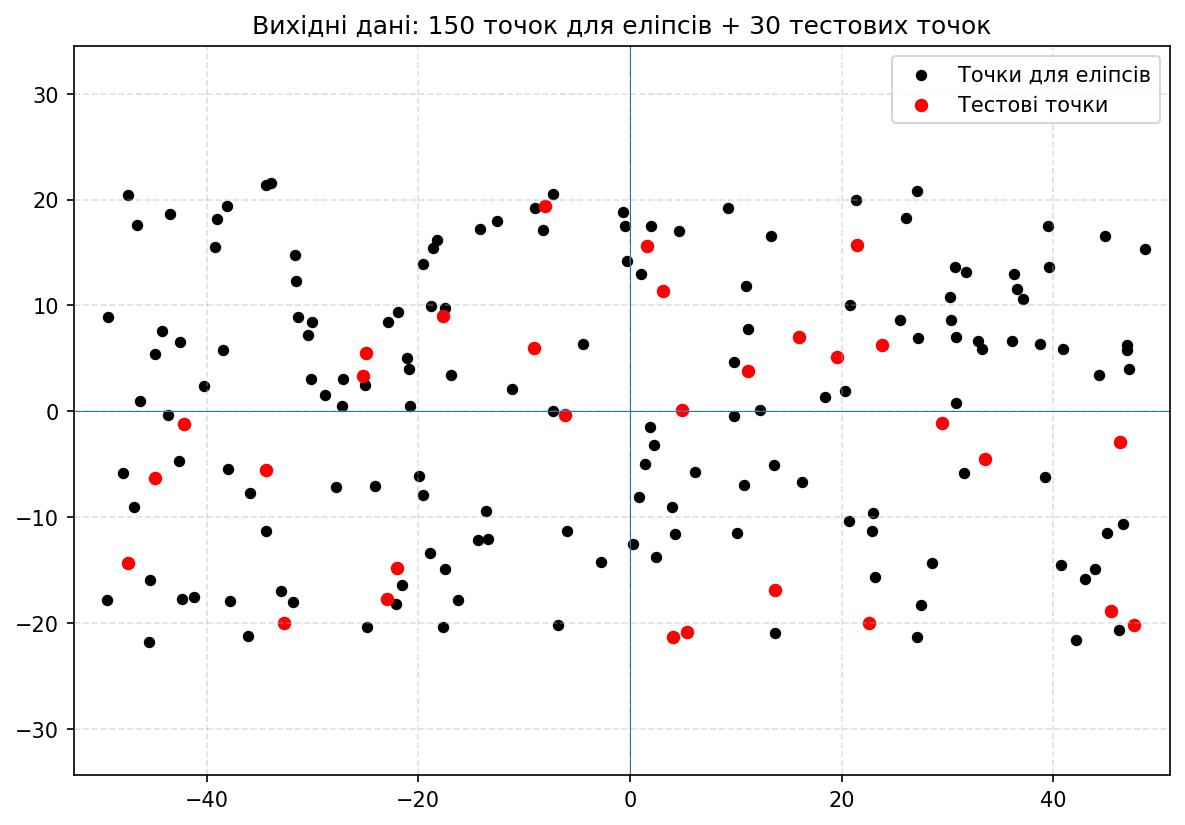
\includegraphics[width=0.8\textwidth]{figures/fig1_input_points.png}
\caption{Вихідні точки: 150 точок для еліпсів (чорні) та 30 тестових точок (червоні)}
\end{figure}

\subsection{Крок 2: Пошук опуклої оболонки та найвіддаленіших точок}

На опуклій оболонці знаходяться дві точки з максимальною відстанню між собою. Це робиться перевіркою всіх пар вершин оболонки.

\textbf{Результат:} 
\begin{itemize}
    \item Знайдено опуклу оболонку з 10 вершинами
    \item Дві найвіддаленіші точки на відстані $d \approx 103.6144$ одиниць
\end{itemize}

\begin{figure}[H]
\centering
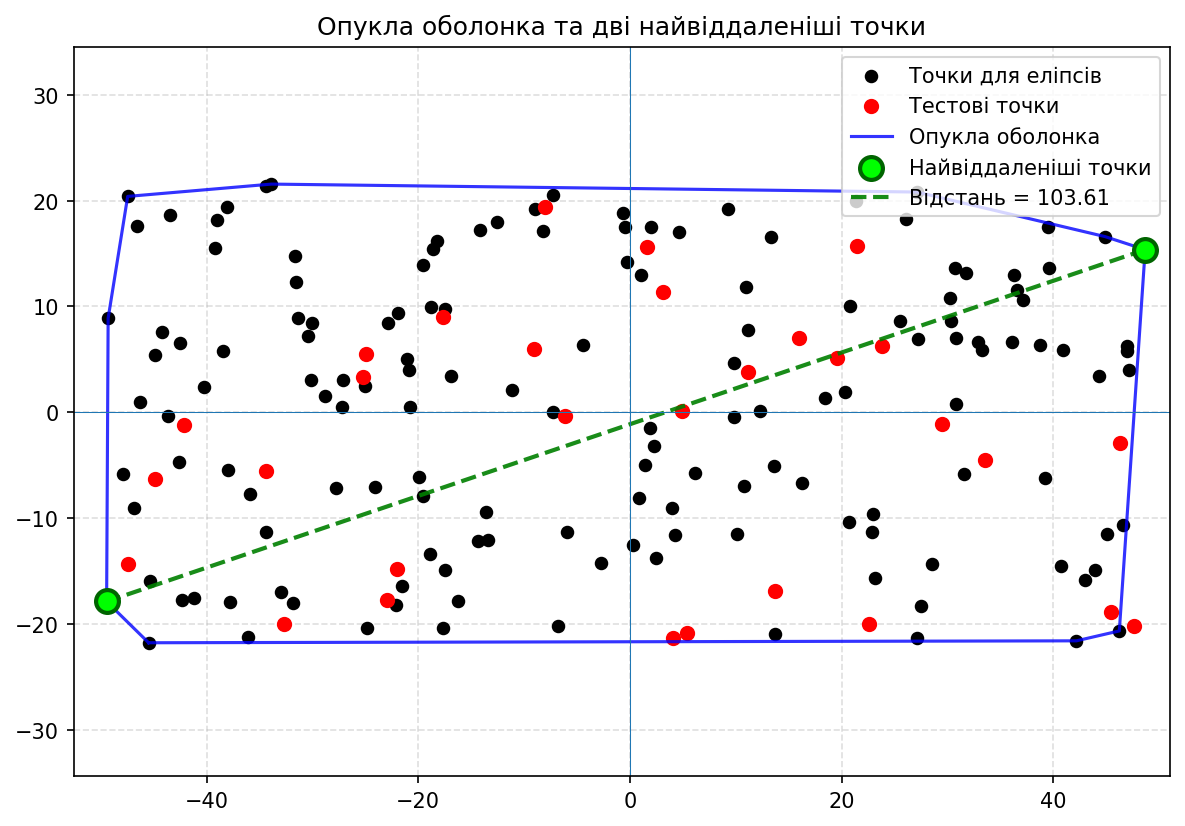
\includegraphics[width=0.8\textwidth]{figures/fig2_convex_hull.png}
\caption{Опукла оболонка (синя лінія) та дві найвіддаленіші точки (зелені)}
\end{figure}

\subsection{Крок 3: Найвіддаленіші точки по різні боки від прямої}

Після потенційного повороту координатної системи знаходяться найвіддаленіші точки вище та нижче горизонтальної прямої.

\begin{figure}[H]
\centering
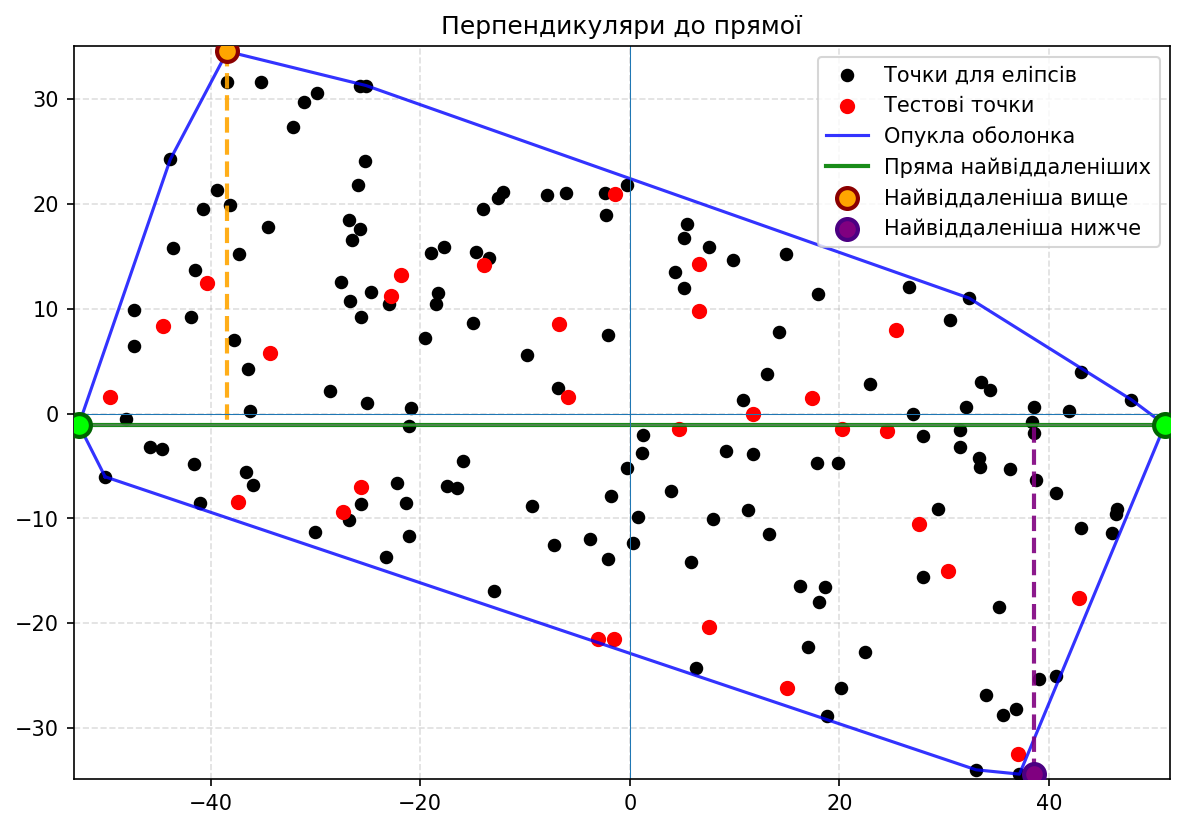
\includegraphics[width=0.8\textwidth]{figures/fig3_perpendiculars.png}
\caption{Перпендикуляри до прямої найвіддаленіших точок}
\end{figure}

\subsection{Крок 4 та 5: Поворот та приведення до квадрату}

Система координат повертається на кут $\theta$ так, щоб пряма найвіддаленіших точок стала горизонтальною. Потім область масштабується до квадратної форми.

\textbf{Параметри масштабування:}
\begin{itemize}
    \item Центр: $(x_c, y_c) \approx (-0.7625, 0.0702)$
    \item Коефіцієнт масштабування: $k \approx 1.5026$
    \item Стиск по осі: $x$
\end{itemize}

\begin{figure}[H]
\centering
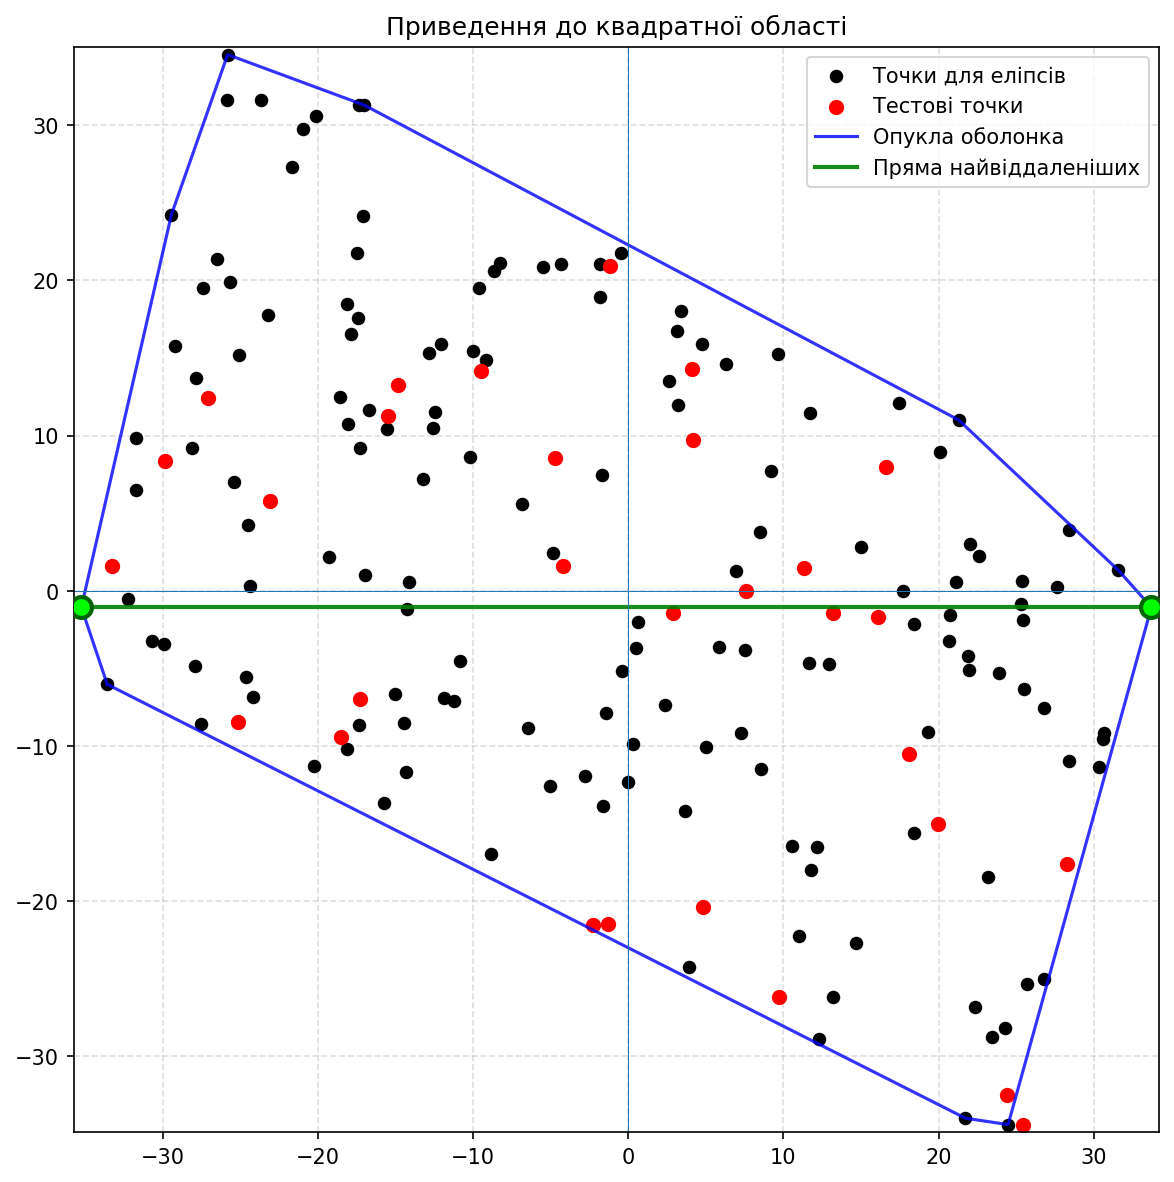
\includegraphics[width=0.8\textwidth]{figures/fig4_square_scaling.png}
\caption{Приведення області до квадратної форми}
\end{figure}

\subsection{Крок 6: Система вкладених кіл}

У центрі квадратної області будується 150 концентричних кіл з радіусами, що відповідають відстаням від центру до кожної точки множини.

\textbf{Статистика радіусів:}
\begin{itemize}
    \item Мінімальний радіус: $r_{min} \approx 2.5123$
    \item Максимальний радіус: $r_{max} \approx 42.7286$
    \item Унікальних кіл: 149
\end{itemize}

\begin{figure}[H]
\centering
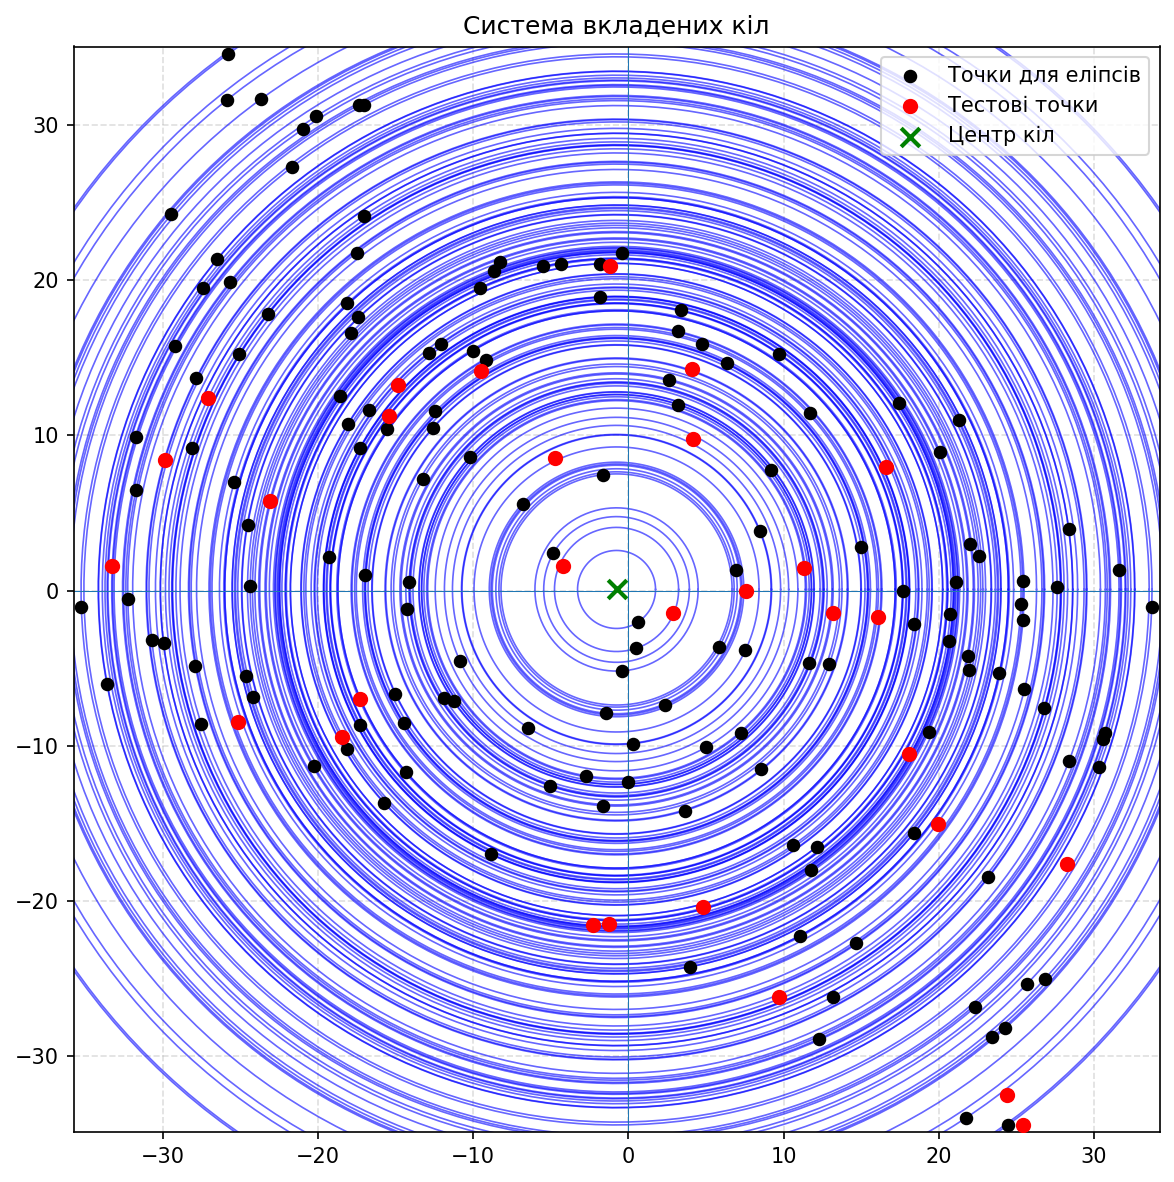
\includegraphics[width=0.8\textwidth]{figures/fig5_nested_circles.png}
\caption{Система вкладених кіл в центрі квадратної області}
\end{figure}

\subsection{Крок 7: Зворотне масштабування та еліпси}

Система кіл перетворюється назад до об'єму, відповідного розтяженню осей. Кола стають еліпсами.

\begin{figure}[H]
\centering
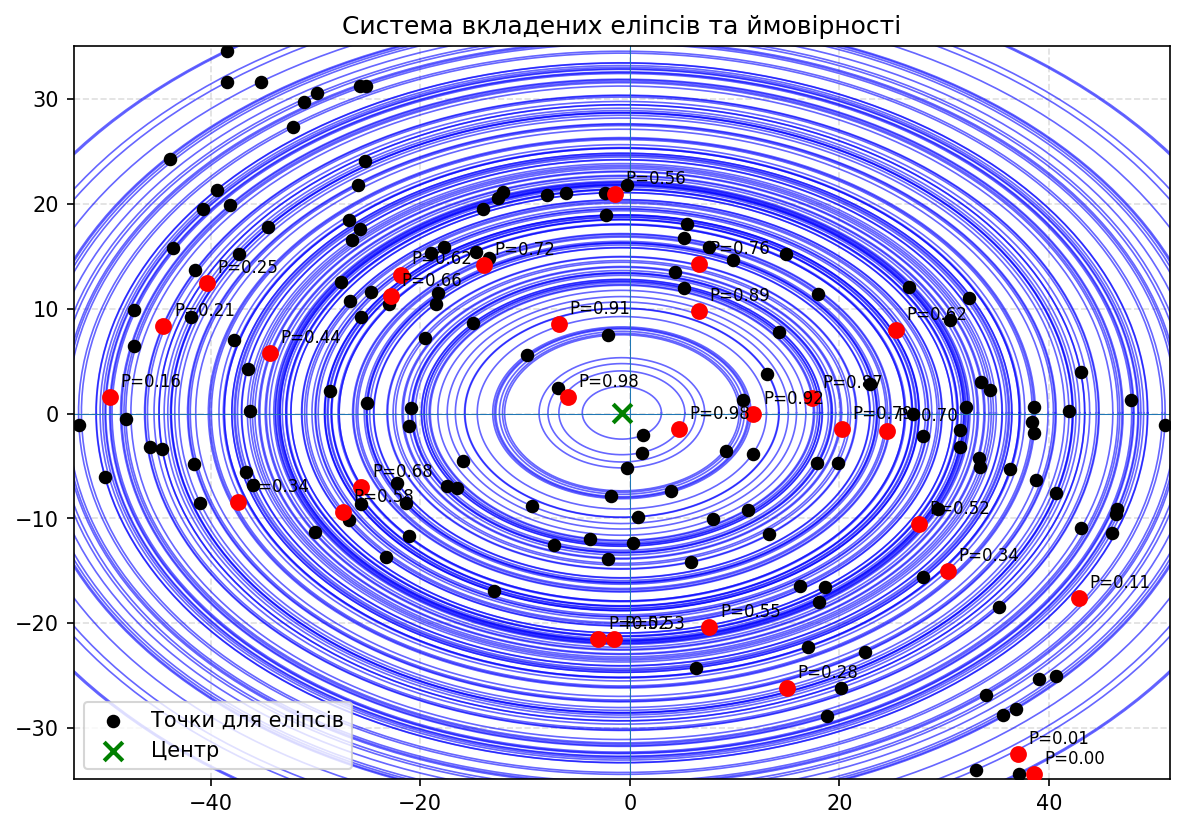
\includegraphics[width=0.8\textwidth]{figures/fig6_nested_ellipses.png}
\caption{Система вкладених еліпсів після зворотного масштабування та ймовірності $P$ для тестових точок}
\end{figure}

\subsection{Крок 8: Розрахунок площ еліпсів}

Для кожного еліпса розраховуються піввісі та площа:

\begin{equation}
a = k \cdot r, \quad b = r, \quad S = \pi \cdot a \cdot b
\end{equation}

\textbf{Статистика площ еліпсів:}
\begin{itemize}
    \item Мінімальна площа: $S_{min} \approx 29.80$ кв. од.
    \item Максимальна площа: $S_{max} \approx 8618.74$ кв. од.
    \item Середня площа: $S_{avg} \approx 2764.87$ кв. од.
\end{itemize}

\begin{figure}[H]
\centering
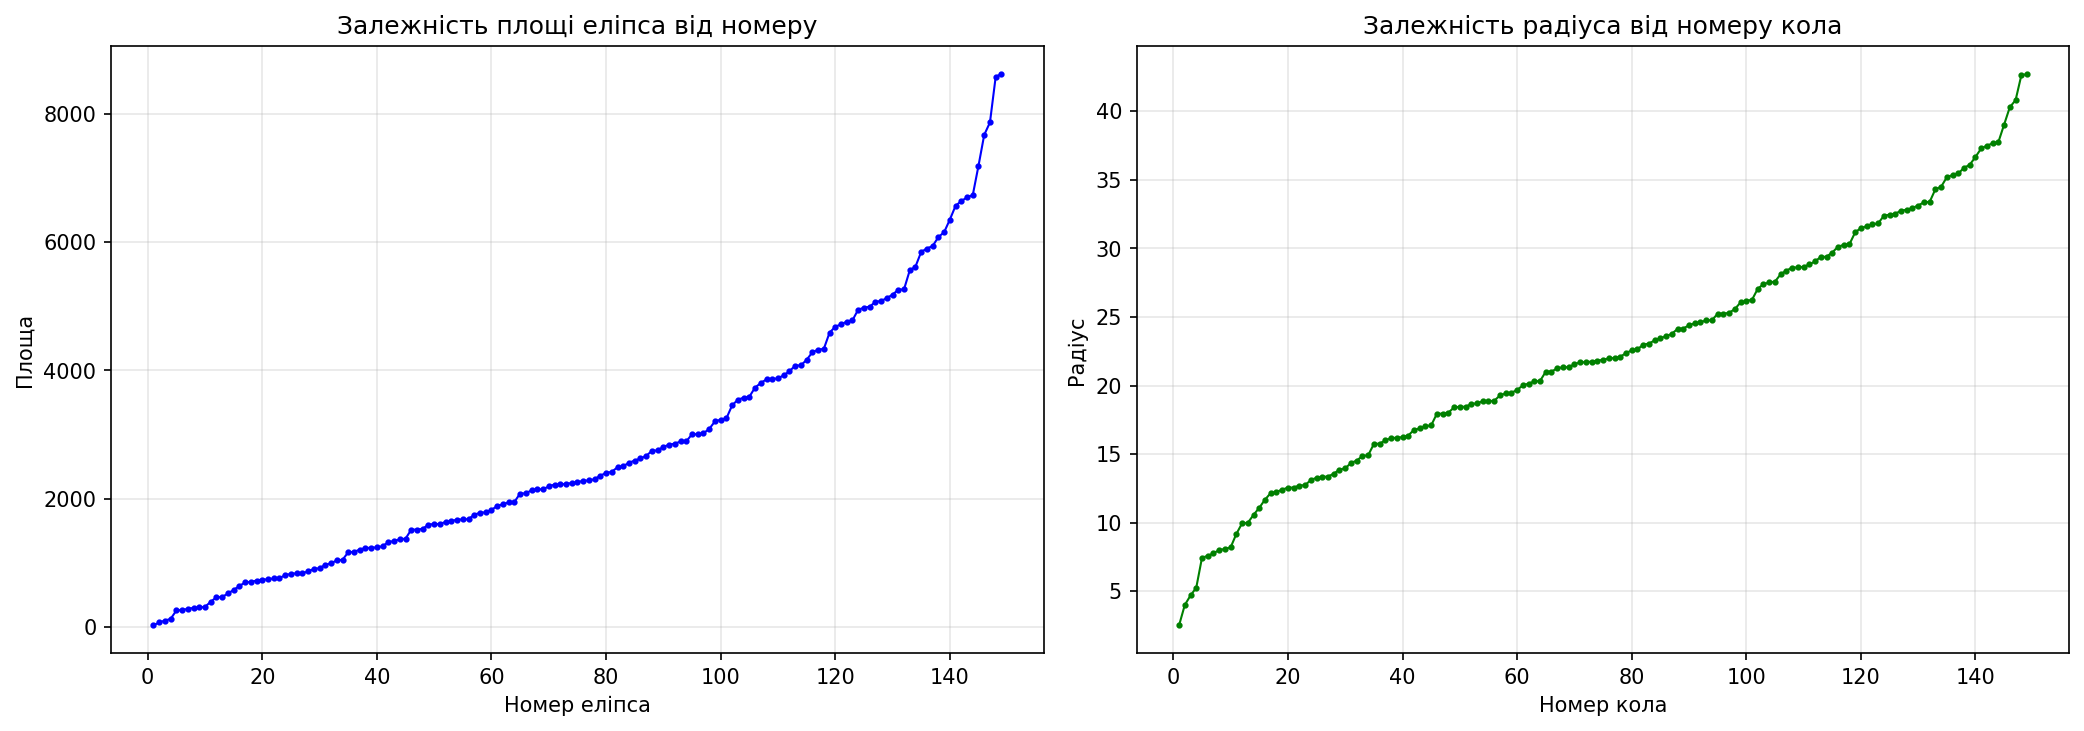
\includegraphics[width=0.95\textwidth]{figures/fig7_ellipse_properties.png}
\caption{Залежність площі еліпса та радіусу від номеру кола}
\end{figure}

%================ РЕЗУЛЬТАТИ ================
\section{Результати класифікації}

\subsection{Таблиця наявності тестових точок у колах}

\begin{table}[H]
\centering
\small
\begin{tabular}{|c|c|c|c|c|c|}
\toprule
\textbf{№} & \textbf{m} & \textbf{P} & \textbf{Статус} & \textbf{x (орг.)} & \textbf{y (орг.)} \\
\midrule
1 & 33 & 0.2119 & $m=33/150$ & -44.83 & -6.34 \\
2 & 136 & 0.8940 & $m=136/150$ & 3.14 & 11.35 \\
3 & 80 & 0.5232 & $m=80/150$ & 4.06 & -21.37 \\
4 & 84 & 0.5497 & $m=84/150$ & 13.74 & -16.89 \\
5 & 44 & 0.2848 & $m=44/150$ & 22.61 & -19.98 \\
6 & 0 & 0.0000 & $m=0/150$ & 47.59 & -20.21 \\
7 & 116 & 0.7616 & $m=116/150$ & 1.63 & 15.64 \\
8 & 109 & 0.7152 & $m=109/150$ & -17.70 & 8.96 \\
9 & 80 & 0.5232 & $m=80/150$ & 29.52 & -1.14 \\
10 & 89 & 0.5828 & $m=89/150$ & -22.92 & -17.70 \\
\midrule
\multicolumn{6}{c}{\textit{(продовження таблиці на наступній сторінці)}} \\
\bottomrule
\end{tabular}
\caption{Результати класифікації тестових точок (1 -- 10)}
\end{table}

\begin{table}[H]
\centering
\small
\begin{tabular}{|c|c|c|c|c|c|}
\toprule
\textbf{№} & \textbf{m} & \textbf{P} & \textbf{Статус} & \textbf{x (орг.)} & \textbf{y (орг.)} \\
\midrule
11 & 149 & 0.9801 & $m=149/150$ & -6.10 & -0.37 \\
12 & 38 & 0.2450 & $m=38/150$ & -42.15 & -1.17 \\
13 & 25 & 0.1589 & $m=25/150$ & -47.46 & -14.38 \\
14 & 18 & 0.1126 & $m=18/150$ & 46.26 & -2.91 \\
15 & 52 & 0.3377 & $m=52/150$ & 33.60 & -4.47 \\
16 & 120 & 0.7881 & $m=120/150$ & 19.60 & 5.10 \\
17 & 139 & 0.9139 & $m=139/150$ & -9.10 & 5.94 \\
18 & 52 & 0.3377 & $m=52/150$ & -32.67 & -20.01 \\
19 & 68 & 0.4437 & $m=68/150$ & -34.36 & -5.52 \\
20 & 94 & 0.6159 & $m=94/150$ & -24.98 & 5.54 \\
\midrule
\multicolumn{6}{c}{\textit{(продовження таблиці на наступній сторінці)}} \\
\bottomrule
\end{tabular}
\caption{Результати класифікації тестових точок (11 -- 20)}
\end{table}

\begin{table}[H]
\centering
\small
\begin{tabular}{|c|c|c|c|c|c|}
\toprule
\textbf{№} & \textbf{m} & \textbf{P} & \textbf{Статус} & \textbf{x (орг.)} & \textbf{y (орг.)} \\
\midrule
21 & 149 & 0.9801 & $m=149/150$ & 4.92 & 0.14 \\
22 & 94 & 0.6159 & $m=94/150$ & 21.46 & 15.69 \\
23 & 133 & 0.8742 & $m=133/150$ & 16.02 & 6.98 \\
24 & 103 & 0.6755 & $m=103/150$ & -22.01 & -14.83 \\
25 & 2 & 0.0066 & $m=2/150$ & 45.49 & -18.89 \\
26 & 107 & 0.7020 & $m=107/150$ & 23.79 & 6.27 \\
27 & 81 & 0.5298 & $m=81/150$ & 5.44 & -20.83 \\
28 & 140 & 0.9205 & $m=140/150$ & 11.17 & 3.77 \\
29 & 86 & 0.5629 & $m=86/150$ & -8.04 & 19.37 \\
30 & 100 & 0.6556 & $m=100/150$ & -25.23 & 3.32 \\
\bottomrule
\end{tabular}
\caption{Результати класифікації тестових точок (21 -- 30)}
\end{table}

\subsection{Статистика результатів}

\begin{table}[H]
\centering
\begin{tabular}{|l|r|}
\toprule
\textbf{Показник} & \textbf{Значення} \\
\midrule
Всього тестових точок & 30 \\
Точок в центрі ($P = 0$) & 1 \\
Точок на краю ($P = 1$) & 0 \\
Точок у середині ($0 < P < 1$) & 29 \\
\midrule
Середня ймовірність & 0.5501 \\
Мінімальна ймовірність & 0.0000 \\
Максимальна ймовірність & 0.9801 \\
\bottomrule
\end{tabular}
\caption{Статистика розподілу тестових точок}
\end{table}

\subsection{Аналіз результатів}

\begin{enumerate}
    \item \textbf{Експансія ймовірностей}: Значення $P$ розподілені від 0.0000 до 0.9801, що демонструє хорошу дискримінацію підходу. Одна точка потрапила в граничний випадок центра ($P=0$).
    
    \item \textbf{Середня ймовірність}: $P_{avg} = 0.5501$.
    
    \item \textbf{Розподіл}: Більшість точок (21 з 30) мають $P > 0.4$, що свідчить про їх концентрацію у зовнішніх шарах еліпсів.
    
    \item \textbf{Граничні випадки}: Точка 6 має $m = 0$ та $P = 0.0000$ (центральний випадок), а найвіддаленіші точки 11 і 21 мають $m = 149$ та $P = 0.9801$.
\end{enumerate}

%================ ВИСНОВКИ ================
\section{Висновки}

\begin{enumerate}
    \item Успішно реалізований 8-кроковий алгоритм побудови системи вкладених еліпсів.
    
    \item Формула $P = \frac{m-1}{n+1}$ забезпечує інтуїтивне представлення ймовірності: точки ближче до центру мають нижчу ймовірність, точки на краї — вищу.
    
    \item Система еліпсів, отримана зворотним масштабуванням, адекватно відображає геометрію вихідної множини точок з урахуванням вертикальної та горизонтальної асиметрії.
\end{enumerate}

%================ ДЖЕРЕЛА ================
\section{Список використаних джерел}

\begin{enumerate}
    \item Graham R. L. An Efficient Algorithm for Determining the Convex Hull of a Finite Planar Set // Information Processing Letters. 1972. Vol. 1, No. 4. P. 132--133.
    \item Convex hull; Graham scan // Wikipedia. URL: \url{https://en.wikipedia.org/wiki/Convex_hull}, \url{https://en.wikipedia.org/wiki/Graham_scan} (дата звернення: 18.03.2026).
    \item Rotation matrix; Affine transformation // Wikipedia. URL: \url{https://en.wikipedia.org/wiki/Rotation_matrix}, \url{https://en.wikipedia.org/wiki/Affine_transformation} (дата звернення: 18.03.2026).
    \item Nonparametric statistics; Empirical distribution function // Wikipedia. URL: \url{https://en.wikipedia.org/wiki/Nonparametric_statistics}, \url{https://en.wikipedia.org/wiki/Empirical_distribution_function} (дата звернення: 18.03.2026).
    \item Ellipse // Wikipedia. URL: \url{https://en.wikipedia.org/wiki/Ellipse} (дата звернення: 18.03.2026).
\end{enumerate}

%================ ДОДАТКИ ================
\appendix

\section{Python код основних функцій}

\subsection{Алгоритм опуклої оболонки}

\begin{lstlisting}[language=Python, basicstyle=\small]
def cross(o, a, b):
    return (a[0] - o[0]) * (b[1] - o[1]) - (a[1] - o[1]) * (b[0] - o[0])

def convex_hull(points):
    pts = np.asarray(points)
    n = len(pts)
    if n < 3:
        return np.arange(n)
    
    idx_ymin = np.argmin(pts[:, 1])
    y_min = pts[:, 1].min()
    cand = np.where(pts[:, 1] == y_min)[0]
    start = cand[np.argmin(pts[cand, 0])]
    
    angles = np.arctan2(pts[:, 1] - pts[start, 1], 
                        pts[:, 0] - pts[start, 0])
    dists = np.sum((pts - pts[start]) ** 2, axis=1)
    order = np.lexsort((-dists, angles))
    order = order[order != start]
    order = np.concatenate([[start], order])
    
    stack = [order[0], order[1]]
    for i in range(2, n):
        k = order[i]
        while len(stack) >= 2 and cross(pts[stack[-2]], 
                    pts[stack[-1]], pts[k]) <= 0:
            stack.pop()
        stack.append(k)
    
    return np.array(stack)
\end{lstlisting}

\subsection{Обчислення ймовірностей}

\begin{lstlisting}[language=Python, basicstyle=\small]
# Probability calculation with edge-case handling
P_test = np.zeros(len(test_sq))
for i in range(len(test_sq)):
    m = max_circle_per_point[i]
    if m == 0:
        P_test[i] = 0.0
    elif m >= n:
        P_test[i] = 1.0
    else:
        P_test[i] = (m - 1) / (n + 1)
\end{lstlisting}

\end{document}
